\documentclass[10pt,twocolumn,letterpaper]{article}

\usepackage{cvpr}
\usepackage{times}
\usepackage{epsfig}
\usepackage{graphicx}
\usepackage{amsmath}
\usepackage{amssymb}

\usepackage{media9}
\usepackage{filecontents}
%\usepackage{geometry}
\usepackage{caption}
\usepackage{subcaption}

% Include other packages here, before hyperref.

% If you comment hyperref and then uncomment it, you should delete
% egpaper.aux before re-running latex.  (Or just hit 'q' on the first latex
% run, let it finish, and you should be clear).
\usepackage[breaklinks=true,bookmarks=false]{hyperref}

\cvprfinalcopy % *** Uncomment this line for the final submission
\def\httilde{\mbox{\tt\raisebox{-.5ex}{\symbol{126}}}}

% Pages are numbered in submission mode, and unnumbered in camera-ready
%\ifcvprfinal\pagestyle{empty}\fi
\setcounter{page}{1}
\begin{document}

%%%%%%%%% TITLE
\title{Volumetric Capture}

\author{Marcel Bruckner\\
{\tt\small email@tum.de}
\and
Kevin Bein\\
{\tt\small email@tum.de}\\
Technical University of Munich
\and
Moiz Sajid\\
{\tt\small moiz.sajid@tum.de}
}

\maketitle
%\thispagestyle{empty}

%%%%%%%%% ABSTRACT
\begin{abstract}
   In this project, our goal is to get realtime 3D mesh reconstruction using a muti-view camera capture setup. We used Intel RealSense cameras for data capture followed by calibration using the marker correspondences. Data is fused into the voxelgrid TSDF followed by Marching cubes for the surface extraction.  
\end{abstract}

%%%%%%%%% BODY TEXT
\section{Introduction}

Volumetric Capture has been a extensively researched topic~\cite{Authors4}.

%------------------------------------------------------------------------
\section{Reconstruction Pipeline}

%-------------------------------------------------------------------------
\subsection{RGB-D Frame Capture}
We used three D415 Intel RealSense cameras for our setup. The reason for using Intel RealSense cameras is good API support that Intel provides for its RealSense cameras. Intel Realsense cameras work on the concept of Active Stereo. The frames from the cameras were time synchronized inorder to get better results for the calibration as well the final mesh reconstruction. For depth preprocessing, we used Threshold Filtering in which the depth of the objects that are certain distance away from the camera get discarded. 

\begin{figure}
  \centering
  \begin{subfigure}[t]{.315\linewidth}
    \centering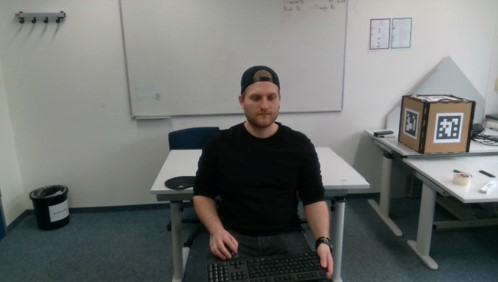
\includegraphics[width=0.9\linewidth]{imgs/rgb}
    \caption{RGB Image}
    \label{fig:rgb}
  \end{subfigure}
  \begin{subfigure}[t]{.315\linewidth}
    \centering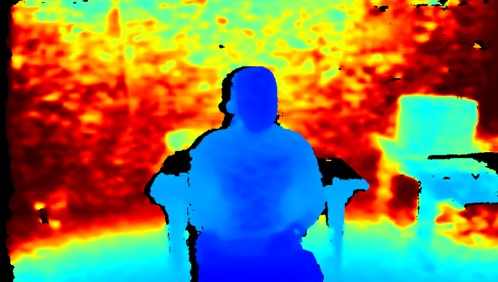
\includegraphics[width=0.9\linewidth]{imgs/depth}
    \caption{Depth Image}
    \label{fig:depth}
  \end{subfigure}
  \begin{subfigure}[t]{.315\linewidth}
    \centering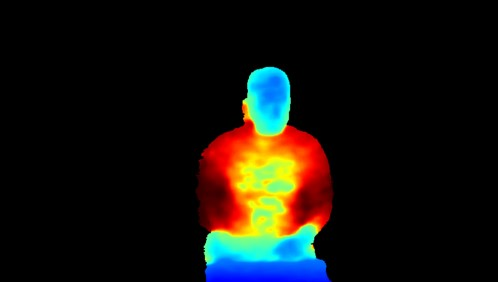
\includegraphics[width=0.9\linewidth]{imgs/threshold}
    \caption{Threshold Filtered Image}
    \label{fig:threshold}
  \end{subfigure}  
  \caption{ }
\end{figure}

For further filtering, we used Hole Filing for ending gaps in the depth images, Spatial Filtering for smoothing the edges and Edge Enhancement Filter. All of these previous filters did not led to any significant improvements. We initally wanted to use four camera but due to bandwidth limitations we were not able to use color and the depth streams from all four cameras. We also had to limit the color and depth frame resolution which in our case was 848 by 480 for the color stream and 848 by 480 for the depth stream.

\begin{figure}[t]
\begin{center}
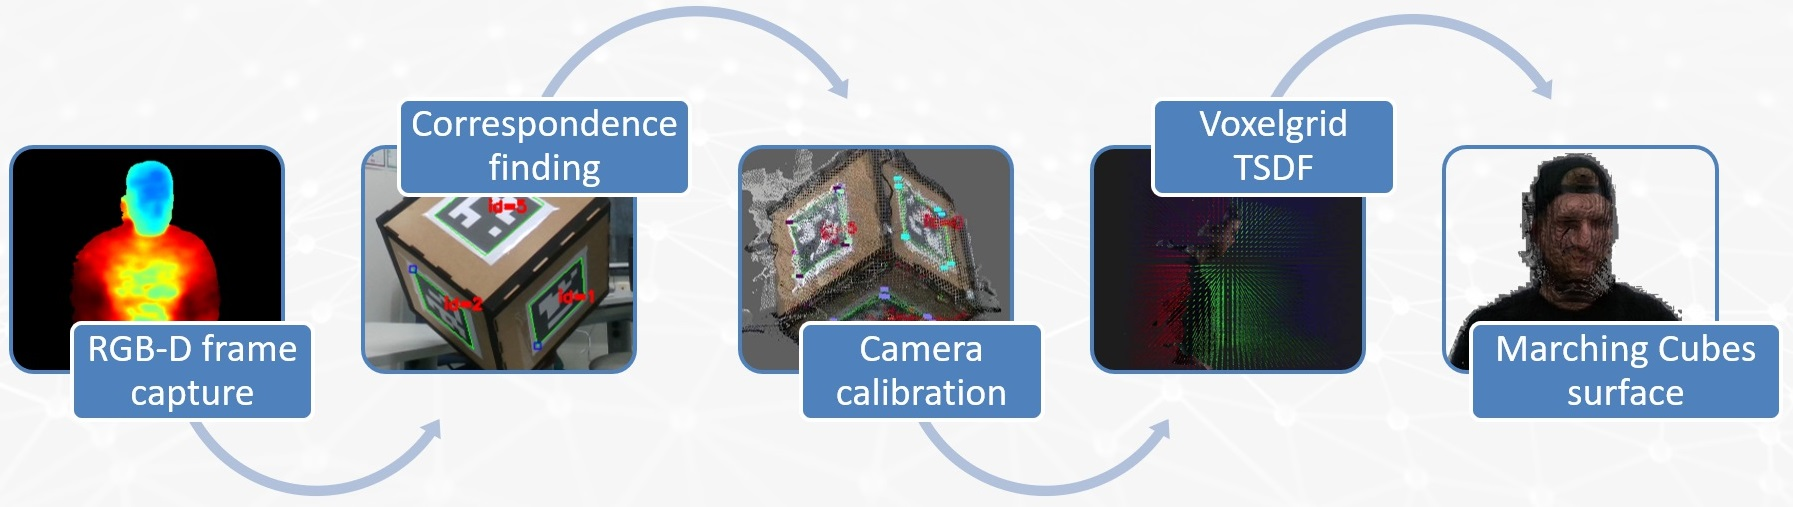
\includegraphics[width=1.0\linewidth]{imgs/pipeline}
\end{center}
 \caption{Reconstruction pipeline used in this project: RGB-D Frame Capture, Correspondence Finding, Camera Calibration, Voxelgrid TSDF, Marching Cubes}
\label{fig:long}
\label{fig:onecol}
\end{figure}
  
%-------------------------------------------------------------------------
\subsection{Correspondence Finding}
For correspondences, we used ArUco markers with each having a unique identifier. The markers were easily detected because we had significant camera view overlap. In the end, we just opted for one marker per side. Once we have the markers, we backproject the correspondences into the pointcloud. We also tried ChArUco markers which is basically a chesboard with arUco markers. But using the ChArUco markers 
%-------------------------------------------------------------------------
\subsection{Camera Calibration}
Once we have the marker locations, we backproject them into the 3D point clouds so that we can estimate the 3D pose between the cameras. 

%-------------------------------------------------------------------------
\subsection{Optimization}
As the camera pose parameters that we got from the camera calibration were not good enough, we used two different approaches namely Procrutes and Point-to-Point correspondence error for optimizing the 3D pose paramters of the cameras further.
 
In the Procrustes algorithm, we compute the vector between the center of gravity for getting the translation component and the Singular Value Decomposition of the known correspondences for getting the rotation component. The alignment we get from Procrustes is not robust enough and hence has a high Mean Squared Error (MSE). In order to further improve the results that we get from Procrustes, we used the Point-to-Point correspondence error. For the Point-to-Point correspondence error, we optimize for the following energy term:

$$
\sum_{i}\sum_{j}\sum_{k} \left\Vert\left(X_{ik} - T_jR_j*X_{jk}\right)\right\Vert_2^2
$$

Further results have been sumarzied in Table~\ref{tab:table1}. One of the difficulties that we faced in camera calibration was visualizing the aligned points for which we had to write our own rendering pipeline in OpenGL. Another difficulty that we faced was with Ceres because we had to get ourselves acquainted with general working of the non-linear optimization framework. 
%-------------------------------------------------------------------------
\subsection{Voxelgrid TSDF}
Once we have these aligned pointclouds, we fuse them into the voxelgrid. We project the voxelgrid into the depth frame of the camera and we calculate the difference by subtracting the voxel depth from the actual depth value as in Equation (\ref{eq1}). For the truncated signed-distance function (tsdf) values we did the weighted averaging using the equation. The tsdf values were truncated between -1 and 1 with values having a negative value inside the surface and positive values outside the surface.

\begin{equation}\label{eq1}
tsdf=z_{voxel} - z_{depth}
\end{equation}

\begin{equation}\label{eq2}
tsdf_{i+1}=\frac{tsdf_{i} * weight}{weight+1}
\end{equation}

Given that we were using a large number of gridpoints, computing tsdf values on the CPU was not feasible. So we had to move our tsdf voxelgrid implementation onto the GPU inorder to achieve realtime results. Since we were already using OpenGL for the rendering pipeline, we decided to use OpenGL Compute Shaders~\cite{Authors1} for parallelizing the tsdf voxelgrid implementation. We also had to find a tradeoff between voxel resolution and frame rate. With a lower voxel resolution, the frame rate dropped because more calculation had to be done. Furthermore, finding a good truncation distance was also very crucial for lowering the artefacts. The Table~\ref{tab:table2} summarizes the time comparisons between different voxel resolution.

\begin{figure}[t]
\begin{center}
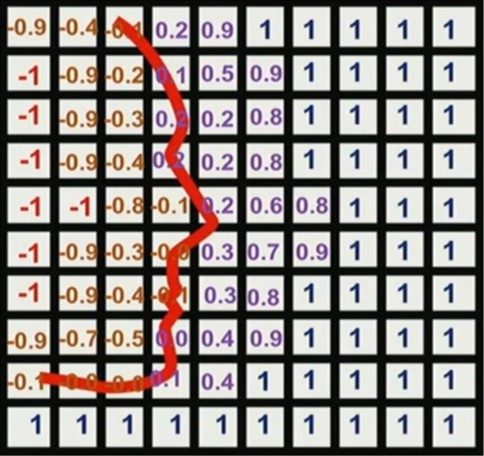
\includegraphics[width=0.6\linewidth]{imgs/tsdf}
\end{center}
 \caption{TSDF Represenation}
\end{figure}

%-------------------------------------------------------------------------
\subsection{Surface Extraction}
For the iso-surface extraction, we used the Marching Cubes algorithm which converts the implicit surface representation to a polygonal mesh. We then iterated over the voxelgrid cells to determine the zero crossings and looked up the triangulation in the Marching Cubes table. This gives us the trianguled mesh as an final output. With a lower voxel resolution and more grid points, we were able to get more finer reconsturction. Again we had to utilize the OpenGL Compute Shader in order to achieve realtime results because the computations on the CPU were really slow.

Intially, we had voxelgrid points that were not initialized because they were outside the camera view. As a result, we had a huge number of artefacts in the final mesh reconstruction which took a lot of time to figure out. We implemented a two pass OpenGL Compute Shader. In the first pass, we counted the number of triangles that will generated and only allocated space for them. In the second pass, we generate the triangles. We do this because the upper bound for the number of generated triangle is five times the number of voxelgrid points. For example if we have 200x200x200 grid points with a 5 millimeter voxel resolution, we roughly had 40 million number of possible triangles. We only generated a fraction of these triangles after the the triangle counting OpenGL Compute Shader pass. For a voxel resolution of 5mm resolution, the Marching Cubes algorithm took 15 milliseconds which was realtime capable. For 3 millimeter resolution, the results were not realtime capable however, we were to get fine mesh reconstructions.  The Table~\ref{tab:table2} summarizes the time comparisons between different voxel resolution. The Table~\ref{tab:table3} summarizes the time comparisons for running Marching Cubes between different voxel resolutions. 

%------------------------------------------------------------------------
\section{Results}
The result was really good with one cameras. But we had some artefacts when we used multiple cameras. Some artefacts were visible around the edges.

\begin{figure}[t]
\begin{center}
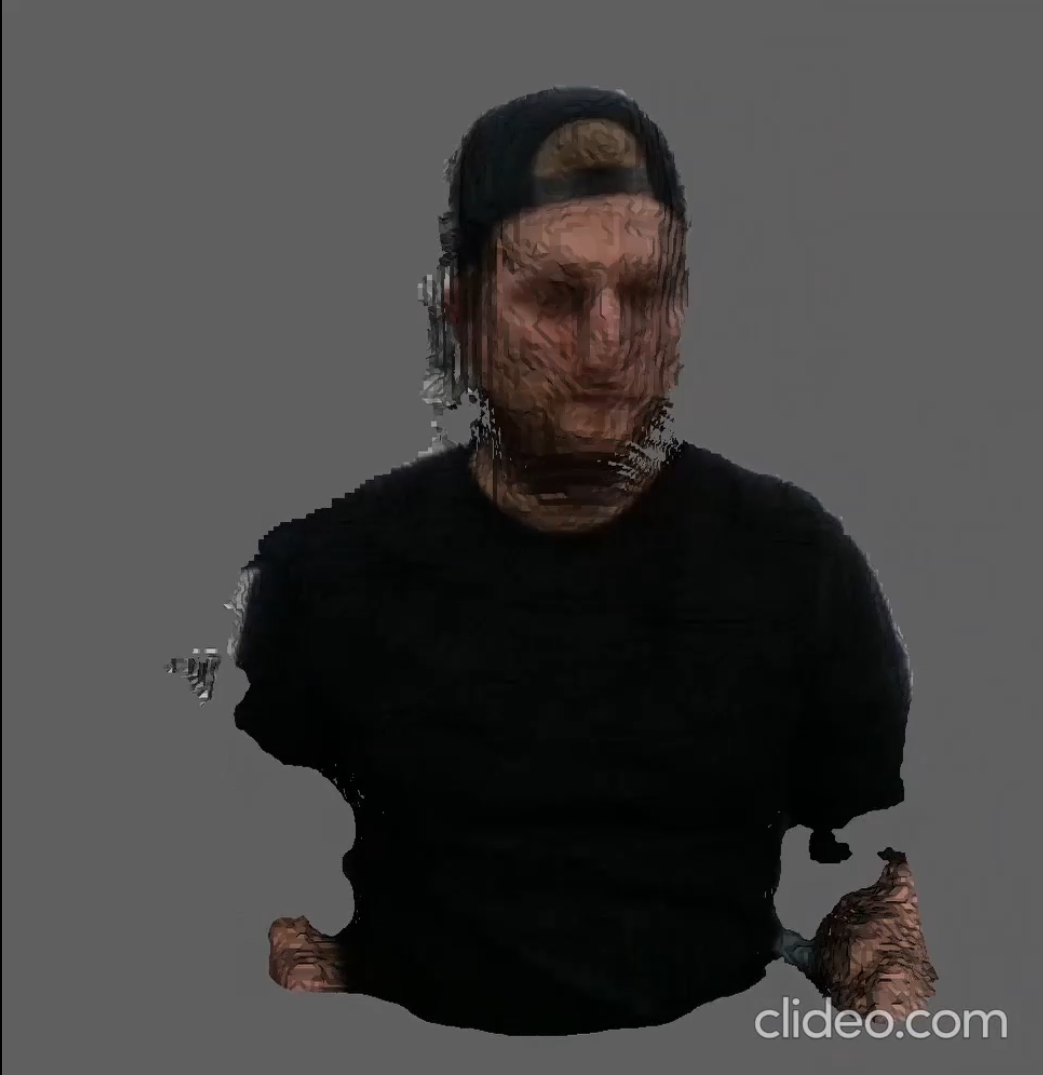
\includegraphics[width=0.65\linewidth]{imgs/res1}
\end{center}
 \caption{Result with using only one camera}
\end{figure}

\begin{figure}[t]
\begin{center}
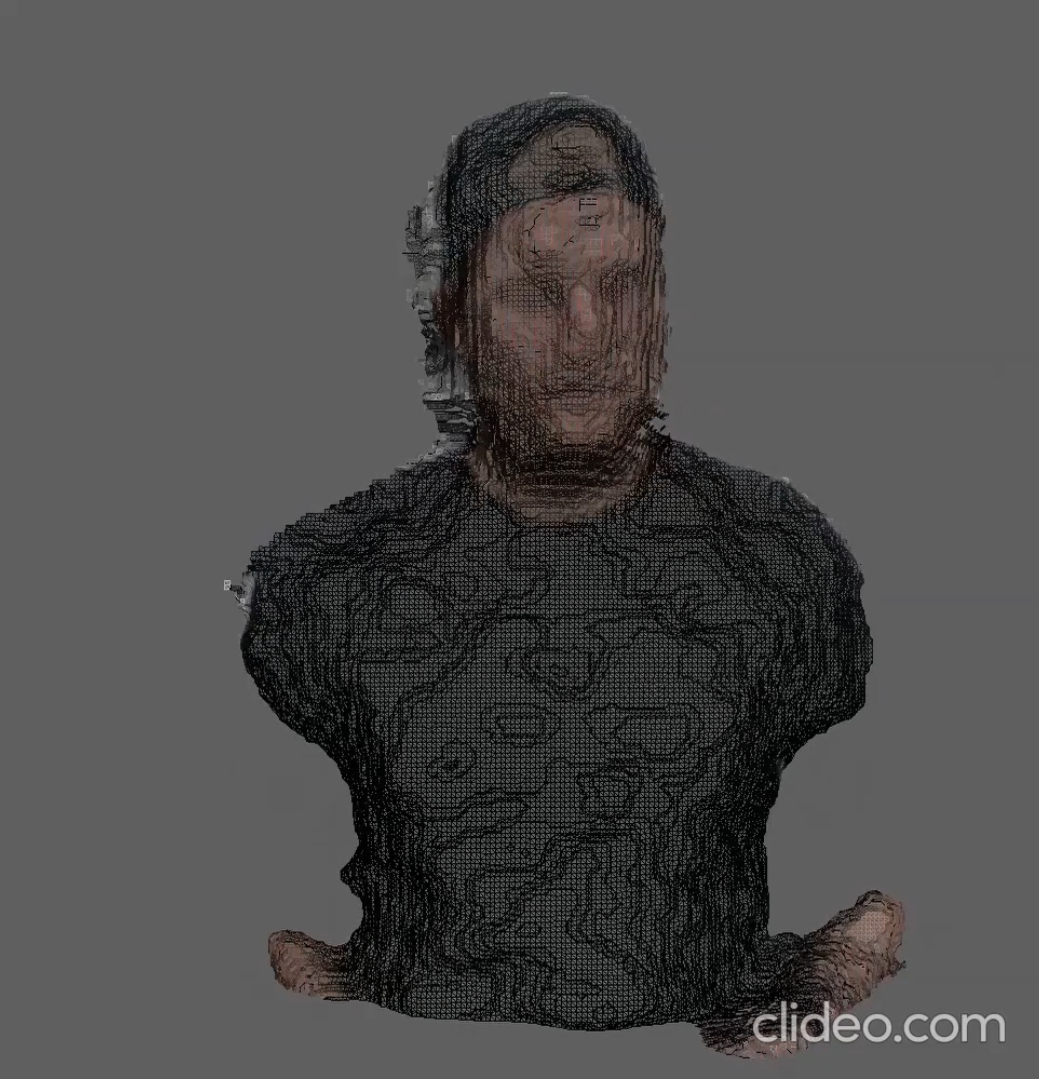
\includegraphics[width=0.65\linewidth]{imgs/res2}
\end{center}
 \caption{Triangulation result with using only one camera}
\end{figure}

\begin{figure}[t]
\begin{center}
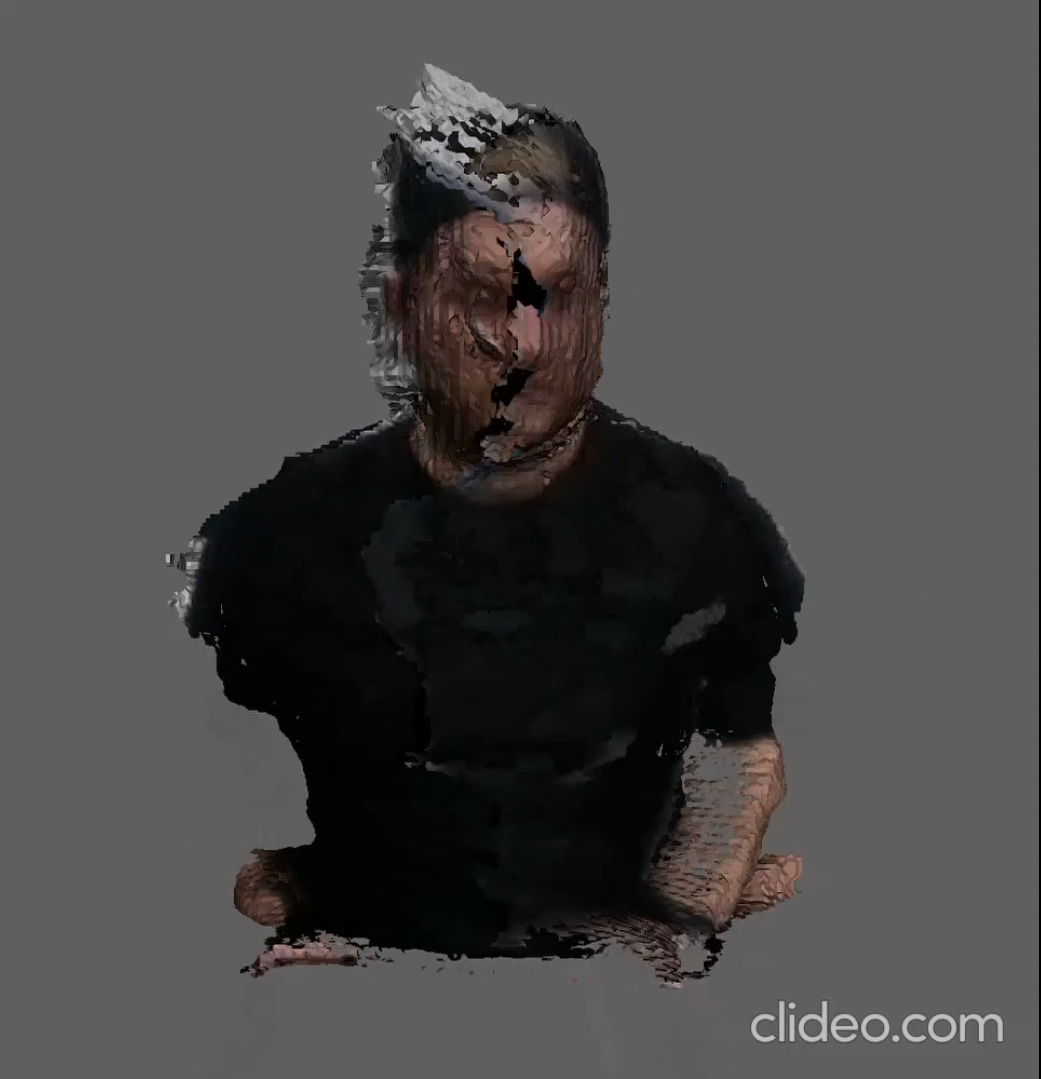
\includegraphics[width=0.65\linewidth]{imgs/res3}
\end{center}
 \caption{Result with using three cameras}
\end{figure}

\begin{table}[h!]
  \begin{center}
    \begin{tabular}{c|c|c|c p{4cm}}
      \textbf{Algorithm} & \textbf{Iterations} & \textbf{Duration [ms]} & \textbf{MSE}\\
      \hline
      Procrustes (A)  & 1 & 8 - 20 & \textless 0.7 - 1.73\\
      Point-to-Point (A) & 1 - 20 & 900 - 1000 & \textless 0.1\\
      Procrustes (C) & 1 & 20 - 40 & 0.25 - 1.29\\
      Point-to-Point (C) & 1 - 20 & 18000 - 22000 & \textless 0.1\\
    \end{tabular}
     \caption{Comparisons between different optimization algorithms in terms of iterations, duration and MSE (Mean Squared Error). A=ArUco and C=ChArUco}
     \label{tab:table1}
  \end{center}
\end{table}

\begin{table}[h!]
  \begin{center}
    \begin{tabular}{c|c|c|c p{4cm}}
      \textbf{Algorithm} & \textbf{Resolution [mm]} & \textbf{Gridpoints} & \textbf{Duration [ms]}\\
      \hline
      All frames & 20 & 125,000 & \textless 1\\
      All frames & 10 & 1,000,000 & \textless 1\\
      All frames & 5 & 8,000,000 & 5\\
      All frames & 4 & 15,625,000 & 20\\
      All frames & 3 & 37,000,000 & 50\\
    \end{tabular}
     \caption{Time comparisons for calculating voxelgrid of different voxel resolutions as well as the number of gridpoints used. The voxelgrid measured 1 meter x 1 meter x 1 meter.}
     \label{tab:table2}
  \end{center}
\end{table}

\begin{table}[h!]
  \begin{center}
    \begin{tabular}{c|c|c p{4cm}}
      \textbf{Resolution [mm]} & \textbf{Duration [ms]} & \textbf{Gridpoints}\\
      \hline
      20 & \textless 1 & 7,000 - 10,000\\
      10 & \textless 1 & 40,000 - 45,000\\
      5 & 15 & 200,000 - 250,000\\
      4 & 35 & 380,000 - 420,000\\
      3 & 80 & 600,000 - 800,000\\
    \end{tabular}
     \caption{Time comparisons for running the Marching Cubes on different voxel resolutions. The number of triangles generated are also displayed.}
     \label{tab:table3}
  \end{center}
\end{table}

%------------------------------------------------------------------------
\section{Future Work}
Since we optimized for pose parameters for a limited number of markers, one of the further improvements that we can do in camera calibration is to use more correspondences which can found for example by using Nearest Neighbor Search and then use the Global Alignment techniques like Iterative Closest Points (ICP).

%------------------------------------------------------------------------
\section{Group Member Contributions}

{\small
\bibliographystyle{ieee_fullname}
\bibliography{egbib}
}

\end{document}
